\documentclass[compress,t,xcolor=table]{beamer}

%\usepackage[table,xcdraw]{xcolor}

%\input{global.macros}
\usepackage[LGR,T1]{fontenc}

\usepackage{pgf}
\usepackage{pgfplots,pgfplotstable}
\usepackage{tikz}
\usetikzlibrary{shapes,backgrounds}
\usetikzlibrary{arrows,shapes,fit,automata,positioning,decorations,calc}
\usetikzlibrary{spy,backgrounds}
\usepackage{siunitx}
\pgfplotsset{compat=1.12}
\usepackage{tabulary}
\usepackage{multirow}
\usepackage{appendixnumberbeamer}
\usepackage{booktabs}

%\usepackage[style=verbose,backend=biber]{biblatex}
%\bibliography{references.bib}


\bibliographystyle{apalike}
\setbeamertemplate{frametitle continuation}[from second]
\setbeamercolor*{bibliography entry title}{fg=black}
\setbeamercolor*{bibliography entry author}{fg=black}
\setbeamercolor*{bibliography entry location}{fg=black}
\setbeamercolor*{bibliography entry note}{fg=black}
\setbeamertemplate{bibliography item}{\insertbiblabel}

\usepackage{listings}
\lstset{language=[LaTeX]TeX,
	numbers=left,
	breaklines=true,
	frame=leftline,
	tabsize=2,
}

\usetheme{Madrid}
\setbeamercovered{transparent}

\definecolor{uoa-blue}{RGB}{3,80,133}
\definecolor{uoa-light-blue}{RGB}{0,154,199}
\definecolor{uoa-grey}{RGB}{230,232,231}

\setbeamercolor{structure}{fg=uoa-blue}

\setbeamertemplate{blocks}[default]
\setbeamercolor{block title}{bg=uoa-blue,fg=white}
\setbeamercolor{block body}{bg=uoa-grey,fg=black}

\setbeamertemplate{title page}[default]

\setbeamertemplate{navigation symbols}{}
%\setbeamertemplate{bibliography item}{\insertbiblabel}

\setbeamertemplate{itemize items}[default]
\setbeamertemplate{enumerate items}[default]

\setbeamertemplate{section in toc}[default]
\setbeamertemplate{subsection in toc}[default]

%\usepackage{fontspec}
%\defaultfontfeatures{Ligatures=TeX}
%\setromanfont{Verdana}

\definecolor{graphFirst}{RGB}{2,136,209} % Light Blue 700
\definecolor{graphSecond}{RGB}{211,47,47} % Red 700
\definecolor{graphThird}{RGB}{245,124,0} % Orange 700
\definecolor{graphFourth}{RGB}{56,142,60} % Green 700
\definecolor{graphFifth}{RGB}{81,45,168} % Deep Purple 700
\definecolor{graphSixth}{RGB}{69,90,100} % Blue Grey 700
\definecolor{graphSeventh}{RGB}{251,192,45} % Yellow 700

\definecolor{backgroundFirst}{RGB}{129,212,250} % Light Blue 200
\definecolor{backgroundSecond}{RGB}{239,154,154} % Red 200
\definecolor{backgroundThird}{RGB}{255,204,128} % Orange 200
\definecolor{backgroundFourth}{RGB}{165,214,167} % Green 200
\definecolor{backgroundFifth}{RGB}{179,157,219} % Deep Purple 200
\definecolor{backgroundSixth}{RGB}{176,190,197} % Blue Grey 200
\definecolor{backgroundSeventh}{RGB}{255,245,157} % Yellow 200

\renewcommand\thefootnote{\textcolor{graphThird}{\arabic{footnote}}}

\newenvironment{myitemize}
{ \begin{itemize}
		\setlength{\itemsep}{10pt}     }
	{ \end{itemize}                  } 


\newenvironment<>{varblock}[2][\textwidth]{%
  \setlength{\textwidth}{#1}
  \begin{actionenv}#3%
    \def\insertblocktitle{#2}%
    \par%
    \usebeamertemplate{block begin}}
  {\par%
    \usebeamertemplate{block end}%
  \end{actionenv}}
  
\AtBeginSection[]
{
	\begin{frame}<beamer>
		\frametitle{Overview}
		\tableofcontents[currentsection]
	\end{frame}
}

\newenvironment{variableblock}[3]{%
	\setbeamercolor{block body}{#2}
	\setbeamercolor{block title}{#3}
	\begin{block}{#1}}{\end{block}}

\usepackage{amsthm}
\setbeamertemplate{theorems}[numbered]

% Keys to support piece-wise uncovering of elements in TikZ pictures:
% \node[visible on=<2->](foo){Foo}
% \node[visible on=<{2,4}>](bar){Bar}   % put braces around comma expressions
%
% Internally works by setting opacity=0 when invisible, which has the 
% adavantage (compared to \node<2->(foo){Foo} that the node is always there, hence
% always consumes space plus that coordinate (foo) is always available.
%
% The actual command that implements the invisibility can be overriden
% by altering the style invisible. For instance \tikzsset{invisible/.style={opacity=0.2}}
% would dim the "invisible" parts. Alternatively, the color might be set to white, if the
% output driver does not support transparencies (e.g., PS) 
%
\tikzset{
	invisible/.style={opacity=0},
	visible on/.style={alt={#1{}{invisible}}},
	alt/.code args={<#1>#2#3}{%
		\alt<#1>{\pgfkeysalso{#2}}{\pgfkeysalso{#3}} % \pgfkeysalso doesn't change the path
	},
}

\tikzset{onslide/.code args={<#1>#2}{%
	\only<#1>{\pgfkeysalso{#2}}
}}
\tikzstyle{highlight}=[red!90, fill=red!5]
\tikzstyle{highlightsource}=[blue!90, fill=blue!5]
\tikzstyle{borderhighlight}=[red!90, text=black, fill=red!5]
\tikzstyle{texthighlight}=[text=red!90, fill=red!5]

\newcommand{\code}[1]{{\small{\texttt{#1}}}}
\newcommand{\todo}[1]{{\color{orange}(TODO: #1)}}

\title[Keyan Monadjem Master's Project]{Synchronous Artificial Neural Networks for Safety Critical Systems}

\author[]{\large Keyan Monadjem}

\institute[University of Auckland]
{
	
\includegraphics[scale=0.3]{fig/UOA-HC-RGB.png}
}

\date[]{
	August 17, 2018
}

\begin{document}

%%%%%%%%%%%%%%%%%%%%%%%%%%%%%%%%%%%%%%%%%%%%%%%%%%%%%%%%%%%%%%%%%%%%%%
\frame{\titlepage}


%%%%%%%%%%%%%%%%%%%%%%%%%%%%%%%%%%%%%%%%%%%%%%%%%%%%%%%%%%%%%%%%%%%%%%
\section{Introduction}

\begin{frame} \frametitle{What is Artificial Intelligence?}
	The aim for machines to intelligently decide the best course of action to meet their respective goals.
	\begin{block}{Machine-based...}
		\begin{myitemize}
			\item Acquisition and Manipulation of Knowledge
			\item Generation and Achievement of Goals
		\end{myitemize}
	\end{block}
\end{frame}

\begin{frame} \frametitle{Are they useful?}
	\centering
	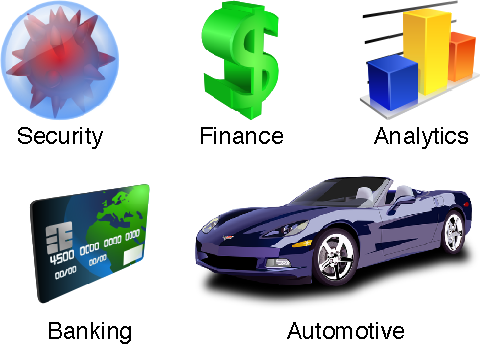
\includegraphics[scale=0.9]{fig/AI-uses.pdf}
	
	\vspace{10mm}
	
	\emph{Image/Pattern Recognition}
\end{frame}

\begin{frame} \frametitle{There are many kinds of AI}
	\begin{block}{(Some) Types}
		\begin{myitemize}
			\item Symbolic AI
			\item Statistical Learning
			\item Sub-symbolic	\begin{myitemize}
				\item Evolutionary Computation
				\item Probabilistic Modelling
				\item \textbf{Artificial Neural Networks (ANNs)}
			\end{myitemize}
		\end{myitemize}
	\end{block}
\end{frame}

\begin{frame} \frametitle{AI is \textit{reactive}...}
	\centering
	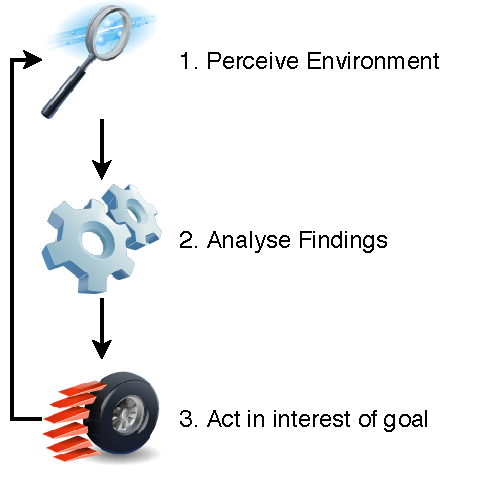
\includegraphics[scale=0.9]{fig/reactive-AI.pdf}
\end{frame}


\begin{frame} \frametitle{Reactive Safety-Critical Systems}
	\centering
	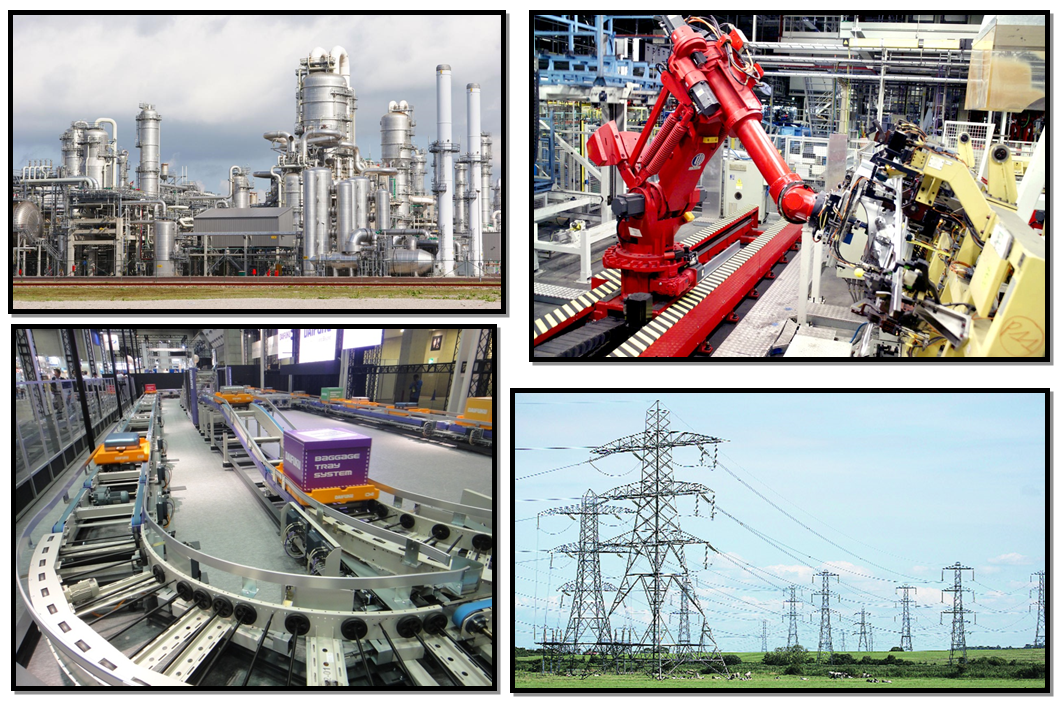
\includegraphics[scale=0.4]{fig/1234.png}
\end{frame}

%\begin{frame} \frametitle{AI Controllers?}
%	\centering
%	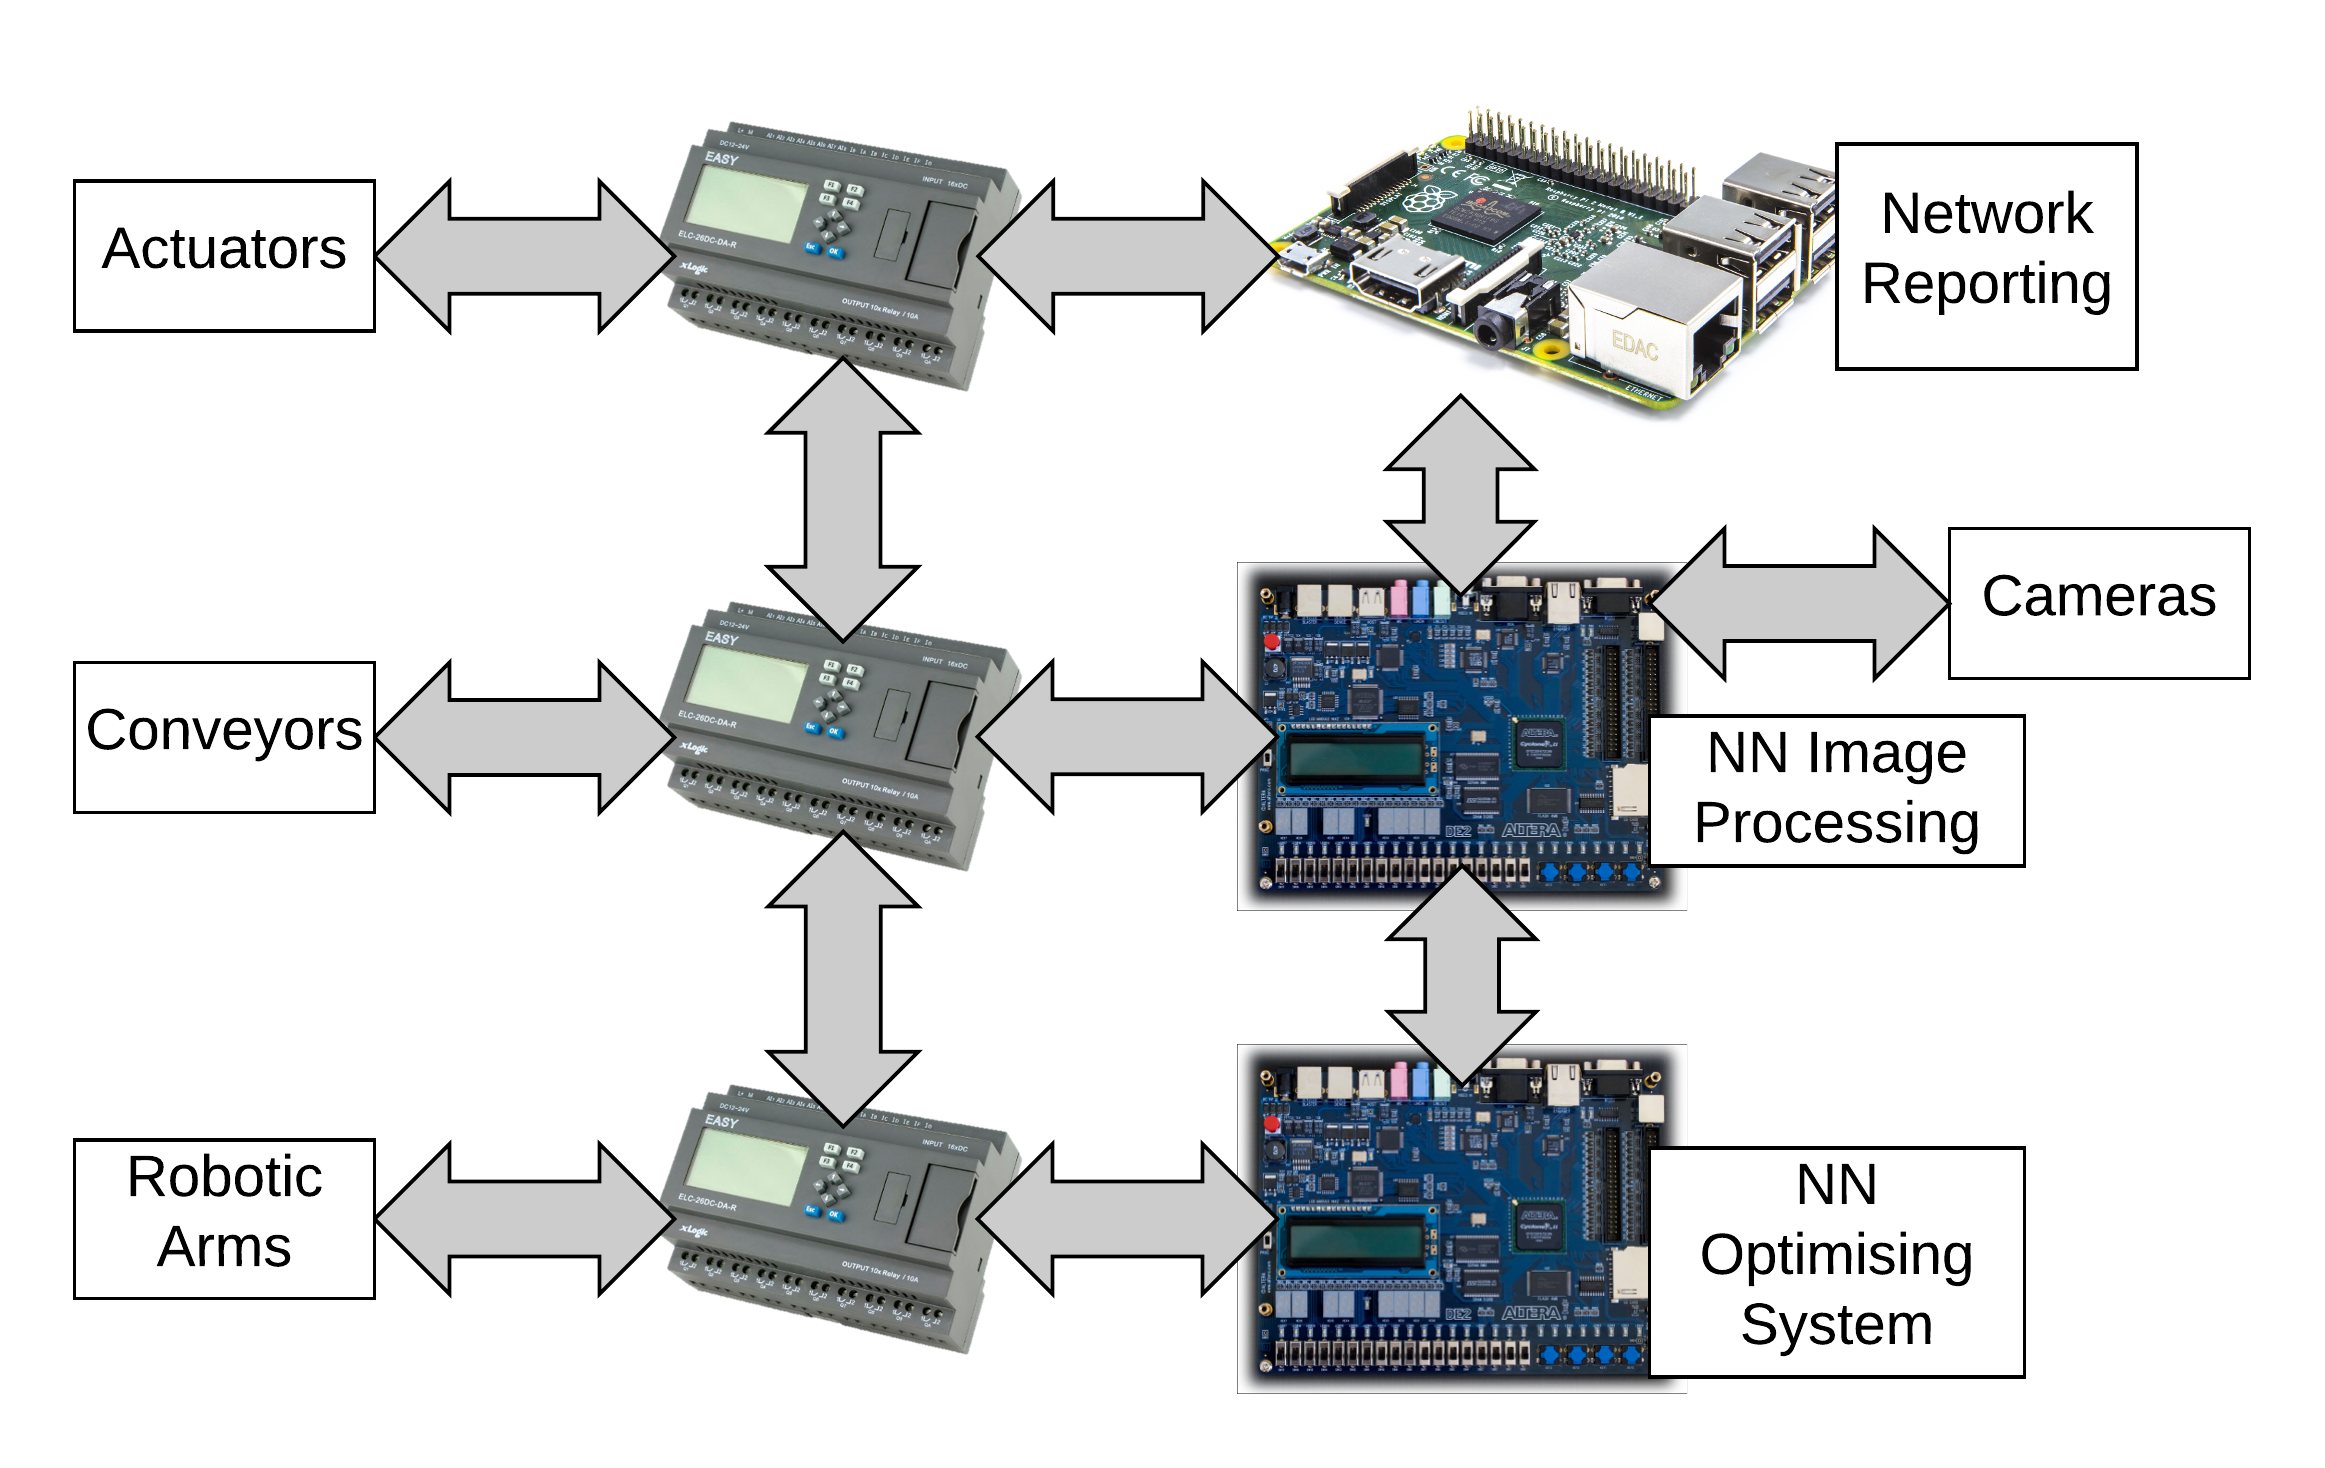
\includegraphics[scale=0.6]{fig/ad-hoc-network.png}
%\end{frame}

\section{Background}

\begin{frame} \frametitle{A brief overview of ML}
	Software that learns data relationships without the software knowing the relationships beforehand.
	\begin{block}
		\centering
		\begin{myitemize}
			\item Decision trees
			\item \textbf{ANNs - deep learning}
			\item Reinforcement learning
		\end{myitemize}
	\end{block}
\end{frame}

\begin{frame} \frametitle{A brief overview of ANNs}
	\begin{myitemize}
		\item Originally designed to model the brain.
		\item One neural network is a group of interconnected nodes, called artificial neurons, which pass signals among themselves.
	\end{myitemize}
	\begin{columns}
		\begin{column}{0.45\linewidth}	
			\begin{figure}[t]
				\centering
				\scalebox{0.5}{\def\layersep{2.25cm}
\def\numInp{4}
\def\numHid{5}
\def\numOut{3}
\begin{tikzpicture}[shorten >=1pt,->,draw=black!100, node distance=\layersep]
	\tikzstyle{every pin edge}=[<-,shorten <=1pt]
	\tikzstyle{neuron}=[circle,fill=black!25,minimum size=20pt,inner sep=0pt]
	\tikzstyle{input neuron}=[neuron, fill=white!100,draw=black];
	\tikzstyle{output neuron}=[neuron, fill=white!100,draw=black];
	\tikzstyle{hidden neuron}=[neuron, fill=white!100,draw=black];
	\tikzstyle{annot} = [text width=4em, text centered]
	
	% Draw the input layer nodes
	\foreach \name / \y in {1,...,\numInp}
	% This is the same as writing \foreach \name / \y in {1/1,2/2,3/3,4/4}
	\node[input neuron, pin=left:Input \y] (I-\name) at (0,-\y) {$i_\y$};
	
	% Draw the hidden layer nodes
	\foreach \name / \y in {1,...,\numHid}
	\path[yshift=0.5cm]
	node[hidden neuron] (H-\name) at (\layersep,-\y cm) {$h_\y$};
	
	% Draw the output layer nodes
	\foreach \name / \y in {1,...,\numOut}
	\node[output neuron, pin={[pin edge={->}]right:Output \y}] (O-\name) at (4.5,-0.25-\y) {$o_\y$};
		
	% Connect every node in the input layer with every node in the
	% hidden layer.
	\foreach \source in {1,...,\numInp}
	\foreach \dest in {1,...,\numHid}
	\path (I-\source) edge (H-\dest);
	
	% Connect every node in the hidden layer with the output layer
	\foreach \source in {1,...,\numHid}
	\foreach \dest in {1,...,\numOut}
	\path (H-\source) edge (O-\dest);
	
	% Annotate the layers
	\node[annot,above of=H-1, node distance=1cm] (hl) {\textit{Hidden Layer}};
	\node[annot,left of=hl] {\textit{Input Layer}};
	\node[annot,right of=hl] {\textit{Output Layer}};
\end{tikzpicture}}
				\caption{Example of an ANN.	\label{fig:ann}}
			\end{figure}
		\end{column}
		\begin{column}{0.45\linewidth}
			\begin{figure}[t]
				\centering
				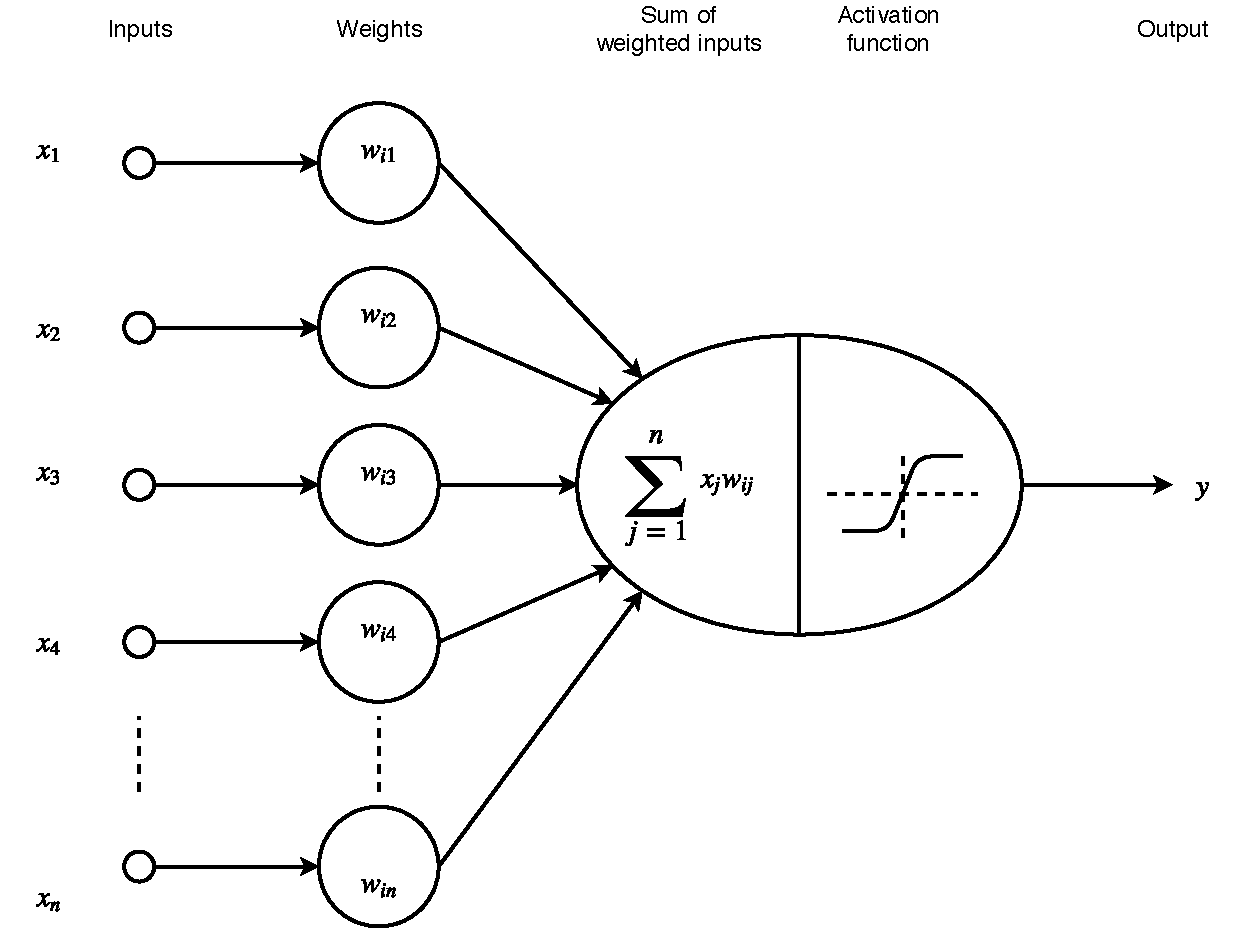
\includegraphics[scale=0.2]{fig/ArtificialNeuron.pdf}
				\caption{Example of an artificial neuron.	\label{fig:neuron}}
			\end{figure}
		\end{column}
	\end{columns}
\end{frame}

\begin{frame} \frametitle{Verified ANNs for safety critical systems}
	\begin{myitemize}
		\item Software/systems based on ML can be very complex.
		\item Not suitable for safety critical systems without validation/verification.
		\item Existing techniques to verify/validate ANNs for safety critical environments (proactive) - not always ideal.
		\item Few solutions for \textit{reactive} safety critical ANNs.
		\item Functional Analysis and formal methods (e.g. \textbf{WCRT}).
		\item \textbf{Runtime Enforcement}.
	\end{myitemize}
\end{frame}

\section{Existing Solutions for Safety-Critical AI Systems}

\begin{frame} \frametitle{Current AI in safety-critical applications}
	\begin{block}{Validation and Verification}
		\begin{myitemize}
			\item Unit testing
			\item Strict guidelines~\nocite{ANNDevModel1999}
			\item Verification algorithms~\cite{safe_verify}\cite{reluplex}\cite{ai2} 
		\end{myitemize}
	\end{block}
\end{frame}

\begin{frame}
	\begin{block}{Safety Critical Artificial Neural Networks (SCANNs) \cite{scann}}
		\begin{myitemize}
			\item Fuzzy Self-Organising Maps (FSOMs)
			\item Rule extraction and insertion
			\item Safety cases
		\end{myitemize}
	\end{block}
\end{frame}

\begin{frame} \frametitle{Why Are Current Implementations \textit{Bad}?}
	\begin{myitemize}
		\item Difficult to formally quantify an ANN.
		\item Verification of ANNs hot topic and highly researched.
		\item Does not address faulty run-time outputs.
	\end{myitemize} 
\end{frame}

\section{Motivating example}
\begin{frame} \frametitle{Uber autonomous vehicle fatal accident} 
	\begin{block}{What happened?}\cite{uber1}
		\begin{myitemize}
			\item Uber autonomous vehicle.
			\item Vehicle collided with jaywalking pedestrian.
			\item \textbf{Fatal}.
		\end{myitemize}
	\end{block}
\end{frame}
\begin{frame}
	\begin{block}{What went wrong?}
		\begin{myitemize}
			\item Pedestrian was sufficiently inebriated.
			\item ANN misclassified the pedestrian \textbf{multiple times}.
			\item Software (AI) trusted over LiDAR readings.
			\item Vehicle did not brake and driver was not paying attention.
			\item Failure on many fronts, including the software of a \textit{safety critical} system.
		\end{myitemize}
	\end{block}
\end{frame}
\begin{frame}\frametitle{Problem Statement}
	How can artificial neural networks utilise synchronous languages such that the safety and performance of safety-critical systems is improved?
\end{frame}

\section{Solution: Utilising Synchronous Semantics}

\begin{frame} \frametitle{Introduction to Synchronous Semantics~\cite{benveniste2003synchronous}}
	\begin{myitemize}
		\item No chance of deadlocks occurring during runtime.
		\item Loops are bounded.
		\item Causality is maintained.
		\item System is deterministic.
		\item Runtime enforcement and observers.
		\item Easier to formally analyse Worst Case Execution Time (WCET) and Worst Case Reaction Time (WCRT).
	\end{myitemize}
\end{frame}

\begin{frame} \frametitle{WCET}
	\begin{myitemize}
		\item Blackbox ANN that "runs fast enough" - not good enough.
		\item WCET of ANNs using formal methods largely unexplored.
		\item WCET analysis is usually measurement-based .
	\end{myitemize}
\end{frame}

\begin{frame} \frametitle{Synchronous Artificial Neural Networks (SANNs)}
	\begin{myitemize}
		\item Created upon the basis of synchronous semantics using Esterel.
		\item Receives all the bonuses of a synchronous language.
		\item Various ANN compositions, both inter-network (meta neural networks) and intra-network (network scheduling).
	\end{myitemize}
	\begin{columns}
		\begin{column}{0.45\textwidth}
			\begin{figure}[h]
				\centering
				\scalebox{0.8}{\begin{tikzpicture}[->,>=stealth',shorten >=1pt,auto,
node distance=2.5cm,
semithick,scale=0.8, transform shape,scale=0.6, font=\huge]

\tikzstyle{every state}=[ellipse, minimum width=2cm, minimum height=1.5cm, text centered, 
fill=blue!20,draw=none,text=black, draw,line width=0.3mm, font=\LARGE]

%start state
\node[state]
(init) 
{$l_i \odot l_h \odot l_o$}; 

\draw[->] (init.south) 
|- ($(init.south) + (0, -0.75cm)$) 
-| ($(init.east) + (0.25cm, 0)$) 
|- ($(init.east) + (0, 1.5cm)$) 
-| (init.north);

\end{tikzpicture}
}
				\caption{Black box execution of an SANN.	\label{fig:sann-bb}}
			\end{figure}
		\end{column}
		%\begin{column}{0.45\textwidth}
		%	\begin{figure}[h]
		%		\begin{lstlisting}[caption={Esterel implementation of black box scheduling},label={lst:bb}]
		%		loop
		%			call run_ANN_i()(?x1, ?x2);
		%			call run_ANN_h()();
		%			emit y(run_ANN_o()());
		%			pause;
		%		pause;
		%		end
		%		\end{lstlisting}
		%	\end{figure}
		%\end{column}
	\end{columns}
\end{frame}

\begin{frame} \frametitle{Black-box scheduling}
	\begin{myitemize}
		\item Single function call to run the entire neural network in one synchronous tick.
		\item Inputs are provided, outputs are returned.
	\end{myitemize}
	\begin{block}{Disadvantages}
		\begin{myitemize}
			\item Function calls from synchronous programs are hardly new.
			\item Iterates through all layers of the Neural Network in one tick - slow.
			\item High WCRT should the system fail.
		\end{myitemize}
	\end{block}
\end{frame}

\begin{frame} \frametitle{Layer by Layer scheduling}
	\begin{myitemize}
		\item Each synchronous tick runs one layer of the neural network
		\item Between layer results are stored to be used in the next tick
		\item Faster WCRT than black box - system can respond between layers
	\end{myitemize}
	\begin{columns}
		\begin{column}{0.45\textwidth}
			\begin{figure}[h]
				\centering
				\scalebox{0.8}{\begin{tikzpicture}[->,>=stealth',shorten >=1pt,auto,
node distance=2.5cm,
semithick,scale=0.8, transform shape,scale=0.6, font=\huge]

\tikzstyle{every state}=[ellipse, minimum width=2.5cm, minimum height=1.5cm, text centered, 
fill=blue!20,draw=none,text=black, draw,line width=0.3mm, font=\LARGE]

%start state
\node[state]
(l0) 
{$l_i$};

\node[state]
(l1) [below of=l0]
{$l_h$}; 

\node[state]
(l2) [below of=l1]
{$l_o$};  

\path[->] (l0) edge (l1);
\path[->] (l1) edge (l2);

\draw[->] (l2.south) 
|- ($(l2.south) + (0, -0.75cm)$) 
-| ($(l2.east) + (1cm, 0)$) 
|- ($(init.east) + (0, 1.5cm)$) 
-| (init.north);

\end{tikzpicture}
}
				\caption{Layer by layer execution of an SANN.	\label{fig:sann-l}}
			\end{figure}
		\end{column}
		%\begin{column}{0.45\textwidth}
		%	\begin{figure}[h]
		%		\begin{lstlisting}[caption={Esterel implementation of layer by layer scheduling},label={lst:l}]
		%		loop
		%			call run_ANN_i()(?x1, ?x2);
		%			pause;
		%			call run_ANN_h()();
		%			pause;
		%			emit y(run_ANN_o()());
		%			pause;
		%		end
		%		\end{lstlisting}
		%	\end{figure}
		%\end{column}
	\end{columns}
\end{frame}

\begin{frame} \frametitle{Neuron by Neuron scheduling}
	\begin{myitemize}
		\item Each artificial neuron created in Esterel.
		\item Each synchronous tick runs one layer of the neural network.
		\item Each layer connected by signals to previous and/or following layers.
		\item Faster WCRT than layer by layer scheduling - less overhead.
	\end{myitemize}
	\begin{columns}
		\begin{column}{0.45\textwidth}
			\begin{figure}[h]
				\centering
				\scalebox{0.8}{\begin{tikzpicture}[->,>=stealth',shorten >=1pt,auto,
node distance=2.5cm,
semithick,scale=0.8, transform shape,scale=0.6, font=\huge]

\tikzstyle{every state}=[ellipse, minimum width=2.5cm, minimum height=1.5cm, text centered, 
fill=blue!20,draw=none,text=black, draw,line width=0.3mm, font=\LARGE]

%start state
\node[state]
(l0) 
{$i_1 \odot i_2$};

\node[state]
(l1) [below of=l0]
{$h_1 \odot h_2 \odot h_3$}; 

\node[state]
(l2) [below of=l1]
{$o_1$};  

\path[->] (l0) edge (l1);
\path[->] (l1) edge (l2);

\draw[->] (l2.south) 
|- ($(l2.south) + (0, -0.75cm)$) 
-| ($(l2.east) + (1cm, 0)$) 
|- ($(init.east) + (0, 1.5cm)$) 
-| (init.north);

\end{tikzpicture}
}
				\caption{Neuron by neuron execution of an SANN.	\label{fig:sann-n}}
			\end{figure}
		\end{column}
		%\begin{column}{0.45\textwidth}
		%	\begin{figure}[h]
		%	\begin{lstlisting}[caption={Esterel implementation of neuron by neuron scheduling},label={lst:n}]
		%		loop
		%			[
		%				call run_ANN_i1()(?x1);
		%				||
		%				call run_ANN_i2()(?x2);
		%			];
		%			pause;
		%			[
		%				call run_ANN_h1()();
		%				||
		%				call run_ANN_h2()();
		%				||
		%				call run_ANN_h3()();
		%			];
		%			pause;
		%				emit y(run_ANN_o1()());
		%			pause;
		%		end
		%	\end{lstlisting}
		%	\end{figure}
		%\end{column}
	\end{columns}
\end{frame}

\begin{frame} \frametitle{Meta Neural Networks}
	\begin{myitemize}
		\item A composition of SANN black boxes or otherwise.
		\item Intricate combinations feasible due to synchronous semantics.
	\end{myitemize}
	\begin{columns}
		\begin{column}{0.45\linewidth}	
			\begin{figure}[t]
				\centering
				\scalebox{0.8}{\begin{tikzpicture}[->,>=stealth',shorten >=1pt,auto,
node distance=3cm,
semithick,scale=0.8, transform shape,scale=0.6, font=\LARGE]

\tikzstyle{every state}=[rectangle, minimum width=2cm, minimum height=1.5cm, text centered, 
fill=blue!20,draw=none,text=black, draw,line width=0.3mm, font=\LARGE]

\tikzstyle{every ellips}=[fill=none,text=black,line=none,font=\LARGE]

%start state
\node[state]
(n1)
{$M_1$}; 

\node[state]
(n2) [below of=n1]
{$M_2$};

\node[state]
(n3) [right of=n1]
{$M_3$};

\node[state]
(n4) [right of=n2]
{$M_4$}; 

\node[state]
(n5) [right of=n3]
{$M_5$};

\node[state]
(n6) [right of=n4]
{$M_6$}; 

\node[state,fill=none, draw=none]
(el1) [right of=n5]
{...};

\node[state,fill=none, draw=none]
(el2) [right of=n6]
{...};

\node[state]
(nn) [right of=el1]
{$M_n$};

\node[state]
(nn1) [right of=el2]
{$M_{n+1}$};

\path[->] (n1) edge (n3);
\path[->] (n1) edge (n4);
\path[->] (n2) edge (n3);
\path[->] (n2) edge (n4);
\path[->] (n3) edge (n5);
\path[->] (n3) edge (n6);
\path[->] (n4) edge (n5);
\path[->] (n4) edge (n6);
\path[-] (n5) edge (el1);
\path[-] (n5) edge (el2);
\path[-] (n6) edge (el1);
\path[-] (n6) edge (el2);
\path[->] (el1) edge (nn);
\path[->] (el1) edge (nn1);
\path[->] (el2) edge (nn);
\path[->] (el2) edge (nn1);


\end{tikzpicture}
}
				\caption{Example meta neural network with parallel SANNs.	\label{fig:meta-complex2}}
			\end{figure}
		\end{column}
		\begin{column}{0.45\linewidth}
			
			\begin{figure}[t]
				\centering
				\scalebox{0.8}{\begin{tikzpicture}[->,>=stealth',shorten >=1pt,auto,
node distance=3cm,
semithick,scale=0.8, transform shape,scale=0.6, font=\LARGE]

\tikzstyle{every state}=[rectangle, minimum width=2cm, minimum height=1.5cm, text centered, 
fill=blue!20,draw=none,text=black, draw,line width=0.3mm, font=\LARGE]

\tikzstyle{every ellips}=[fill=none,text=black,line=none,font=\LARGE]

%start state
\node[state]
(n1)
{$M_1$}; 

\node[state]
(n2) [below of=n1]
{$M_2$};

\node[state]
(n3) [right of=n1, yshift=-1.5cm]
{$M_3$};

\node[state]
(n4) [right of=n3, yshift=1.5cm]
{$M_4$};

\node[state]
(n5) [below of=n4]
{$M_5$};

\node[state]
(n6) [right of=n4, yshift=-1.5cm]
{$M_6$};

\node[state,draw=none,fill=none]
(el1) [right of=n6, yshift=1.5cm]
{...}; 

\node[state,draw=none,fill=none]
(el2) [below of=el1]
{...}; 


\path[->] (n1) edge (n3);
\path[->] (n2) edge (n3);
\path[->] (n3) edge (n4);
\path[->] (n3) edge (n5);
\path[->] (n4) edge (n6);
\path[->] (n5) edge (n6);
\path[->] (n6) edge (el1);
\path[->] (n6) edge (el2);

\end{tikzpicture}
}
				\caption{Example meta neural network with some parallel SANNs.	\label{fig:meta-complex1}}
			\end{figure}
		\end{column}
	\end{columns}
\end{frame}

\begin{frame} \frametitle{Runtime Enforcement~\cite{SyncRTE2017}}
	\begin{myitemize}
		\item Monitors and corrects a system's I/O.
		\item Cannot delay events or block execution.
		\item E.g. enforce that the vehicle will brake, instead of accelerating, when a collision could occur.
	\end{myitemize}
	\begin{block}{Observers}
		\begin{myitemize}
			\item Statically specify properties of a program.
			\item Verification for synchronous languages.
		\end{myitemize}
	\end{block}
\end{frame}

\begin{frame} \frametitle{Safe Neural Networks (SNNs)}
	\begin{myitemize}
		\item Synchronous Artificial Neural Network (SANN) encapsulated by Runtime Enforcement (RE).
		\item SANN I/O monitored and enforced to be \textit{safe}.
		\item SNN is entirely synchronous and time analysable.
		\item SNN is formally defined (Definition ~\ref{def:ssann}).
	\end{myitemize}
\end{frame}

\begin{frame} \frametitle{Safe Neural Networks (SNNs) - Definition}
	\begin{definition}
		\label{def:ssann}
		An SNN is formalised as a tuple $S = \langle I, O, \varphi_I, \varphi_O, L, \gamma, \alpha  \rangle$, where:
		\begin{itemize}
			\item $I$ is a finite collection of input variables with
			its domain being $\mathbf{I} = \mathbb{R}^n$.
			\item  $O$ is a finite collection of  output variables with
			its domain being $\mathbf{O} = \mathbb{R}^m$.
			\item $\varphi_I$ is an input safety policy specifying the safe behaviour of inputs $I$.
			\item $\varphi_O$ is an output safety policy specifying the safe behaviour of input-outputs $I \times O$.
			\item $L$ denotes a set of ANN layers $\{l_1, l_2, ..., l_k\}$.
			\item $\gamma: I_l \rightarrow O_l$ is the non-linear activation function that provides the behaviour of a given layer, i.e. when provided inputs $I_l$, the layer produces outputs $O_l$.
			\item $\alpha: l_k \rightarrow l_{k+1}$ is the layer-to-layer mapping function
			that maps the outputs of a given layer to the inputs of the following layer.
		\end{itemize}
	\end{definition} 
\end{frame}

\begin{frame} \frametitle{Safe Neural Networks (SNNs) - AV as a SNN}
	\begin{itemize}
		\item $I=\langle S, P, O_{1}, O_{1_S}, O_{1_D} ..., O_{5}, O_{5_S}, O_{5_D} \rangle$, i.e. the 17 different fixed-point integer inputs to the controller ANN.
		\item $O = \langle A, B_S, B_H \rangle$ are the three different fixed-point integer outputs which represent the different actions (and the confidence in the action) that can be taken by the AV at any given time.
		\item $\varphi_I = \varphi_{av_I} = \varphi_{cnn_I} \wedge \varphi_{ped_I} \wedge \varphi_{car_I} \wedge \varphi_{drive_I}$, i.e. the complete set of policies projected on inputs $I$. Once combined, they ensure the safety of the CNN ensemble and LiDAR outputs (i.e. the controller's inputs).
		\item $\varphi_O = \varphi_{av} = \varphi_{cnn} \wedge \varphi_{ped} \wedge \varphi_{car} \wedge \varphi_{drive}$, i.e. the complete set of policies ensuring the safety of the controller. Once combined, they prevent collisions with pedestrians, other vehicles and maintain that the car drives consistently and within the law.
		\item $L = \{l_i, l_h, l_o, l_{pp}\}$, are the four layers of the controller ANN, i.e. the input layer, hidden layer, and output layer of the MLP; and the post processing layer of the controller.
	\end{itemize}
\end{frame}

\section{Working example}
\begin{frame} \frametitle{System Simulation: Autonomous Vehicle (AV)}
	\begin{myitemize}
		\item Enforcer lies between the controller and the plant.
		\item Plant consists of sensors and actuators.
		\item Sensors: LiDAR and cameras
		\item Actuators: Motors and brakes (drive and stop)
	\end{myitemize}
\end{frame}

\begin{frame} \frametitle{AV System Sensor Diagram}
	\begin{figure}[t]
		\centering
		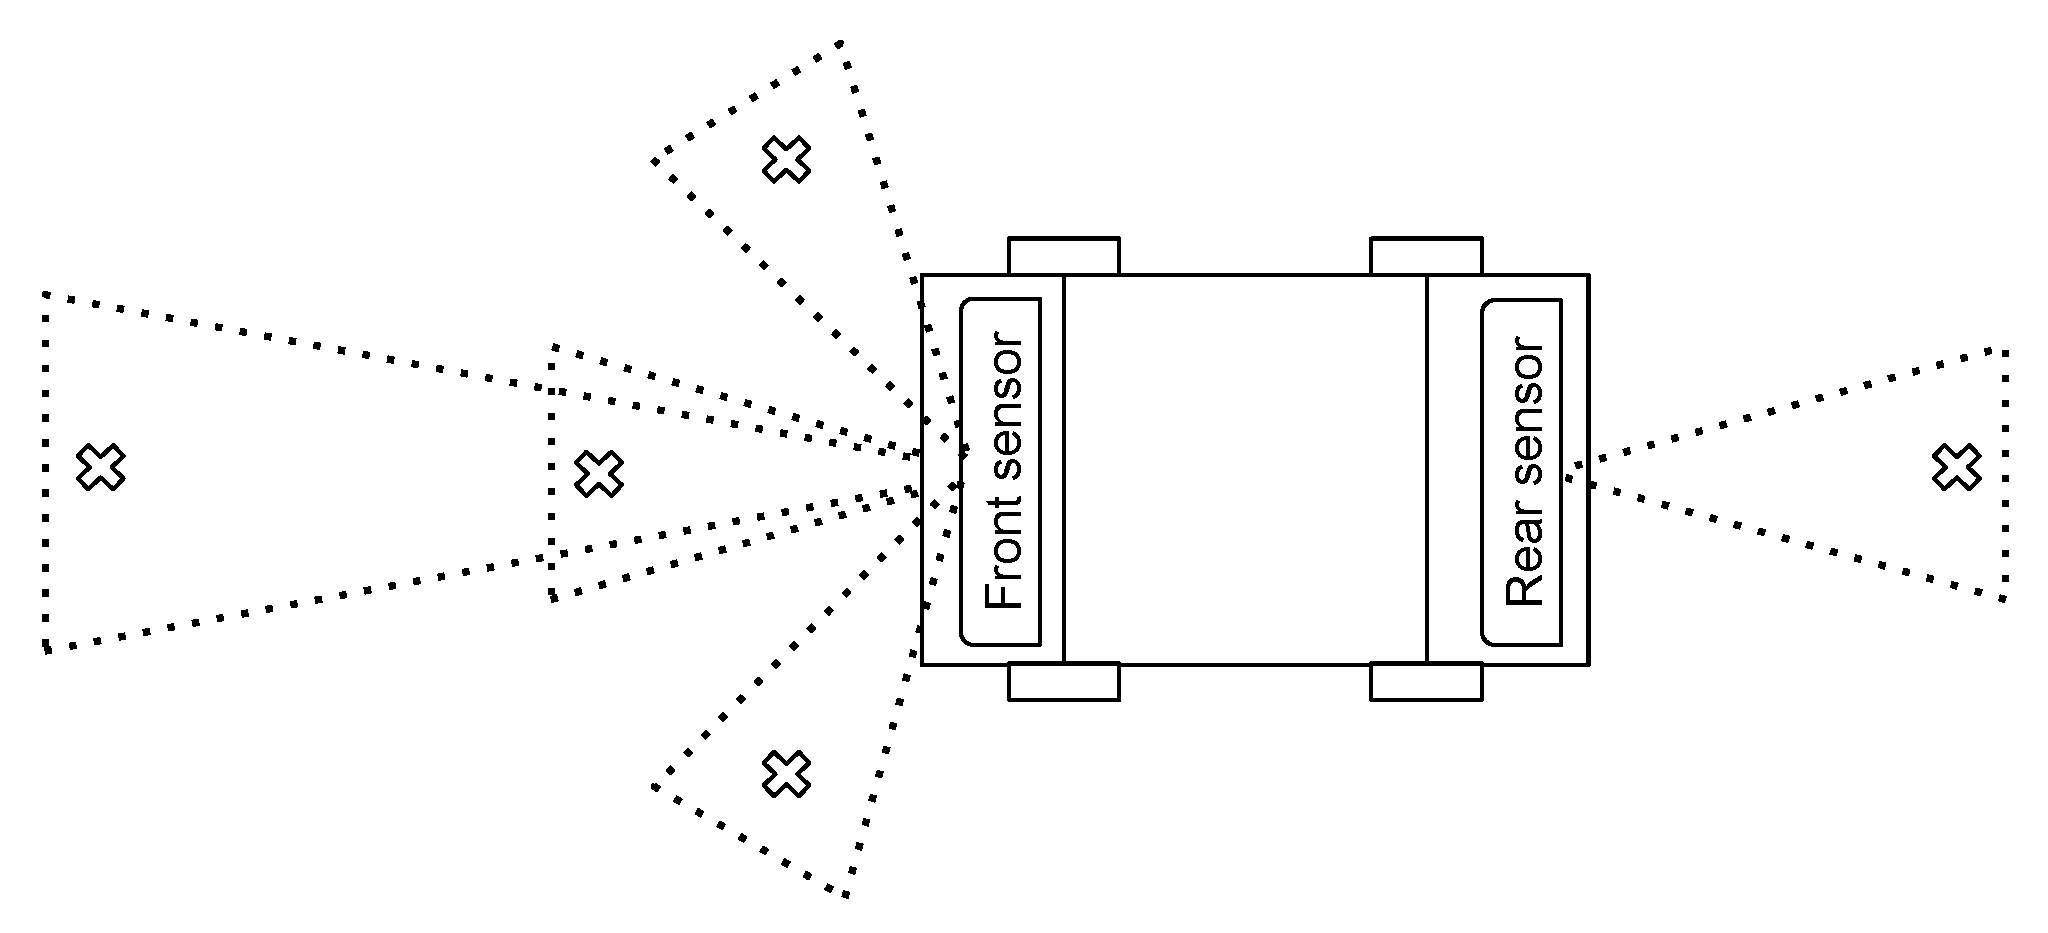
\includegraphics[width=\linewidth]{fig/AV.pdf}
		\caption{Sensor diagram for the AV safety system. \label{fig:car}}
	\end{figure}
\end{frame}
\begin{frame} \frametitle{AV System Block Diagram}
	\begin{figure}[t]
		\centering
		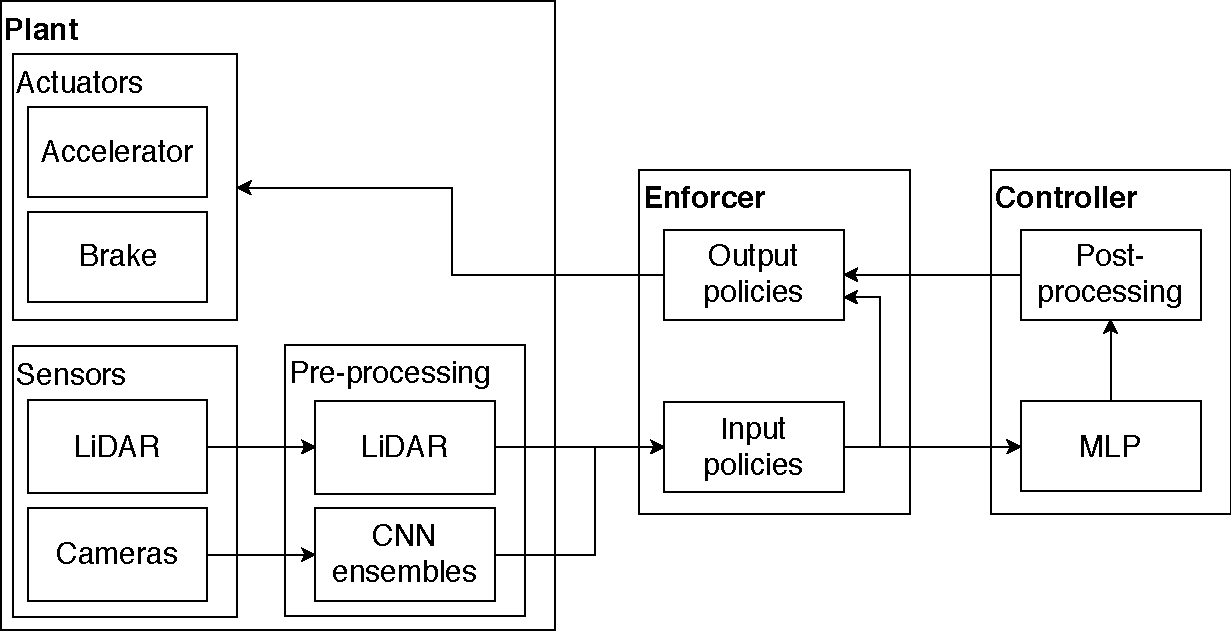
\includegraphics[width=\linewidth]{fig/AV-sys.pdf}
		\caption{Block diagram for the AV safety system. \label{fig:ubersys}}
	\end{figure}
\end{frame}

%\begin{frame} \frametitle{System Simulation: (AV)}
%	\begin{myitemize}
%		\item System too big and diverse to fully replicate.
%		\item Need partial simulation.
%		\item Ensemble must be trained off of a realistic data set
%		\begin{itemize}
%			\item VOC image dataset 2008. \cite{voc2008}
%		\end{itemize}
%		\item LiDAR must be simulated
%		\begin{itemize}
%			\item KITTI autonomous vehicle dataset. \cite{kitti}
%			\item Hours of data driving an autonomous vehicle.
%			\item LiDAR, cameras and GPS.
%		\end{itemize}
%	\end{myitemize}
%\end{frame}

\begin{frame} \frametitle{Runtime Enforcement}
	\begin{figure}[t]
		\centering
		\scalebox{1}{

\begin{tikzpicture}[>=stealth',shorten >=1pt,auto,node distance=4.5 cm, scale = 1, transform shape]

\tikzstyle{accept} = [draw=blue!75,fill=blue!20]
\tikzstyle{violate} = [draw=red!75,fill=red!20]

\node[initial,state, accepting, accept] (A) {$q_{drive}$};
\node[state, accepting, accept] (B) [right of=A] {$q_{brake}$};
\node[state, violate]         (C) [right of=B]  {$q_v$};

\path[->] 
		(A) edge [loop above]       node [above, xshift=-1em]  
		{
			\scriptsize$\let\scriptstyle\textstyle\substack{\overline{B_H}~\&~ \overline{(B_S~\&~P)}, \\ t := 0}$
		} (A)
		
		(A) edge [bend left=45]		node [above]  
		{
			\scriptsize$\let\scriptstyle\textstyle\substack{B_H~|~(B_S~\&~P), \\ t := 0}$
		} (B)
	
		(A) edge [bend right=70]	node [above]  
		{
			\scriptsize$\let\scriptstyle\textstyle\substack{\sum\textbackslash \Big((\overline{B_H}~\&~\overline{(B_S~\&~P)})~|\\~B_H~|~(B_S~\&~P)\Big)}$
		} (C)
	
		(B) edge [loop above]		node [above, xshift=2em]  
		{
			\scriptsize$\let\scriptstyle\textstyle\substack{(t < T_{lim}~|~B_H~|~B_S) \\~\&~\overline{A}}$
		} (B)
	
		(B) edge [left]				node [below]  
		{
			\scriptsize$\let\scriptstyle\textstyle\substack{\{t >= T_{lim}~\& \\ A~\&~\overline{B_H}~\&~\overline{(B_S~\&~P)}}$
		} (A)
		
		(B) edge [right]			node [below]  
		{
			\scriptsize$\let\scriptstyle\textstyle\substack{\sum\textbackslash \Big(t < T_{lim}~|~B_H~|~B_S|\\(t >= T_{lim}~\& \\ A~\&~\overline{B_H}~\&~\overline{B_S \& P})\Big)}$
		} (C)
	
		(C) edge [loop above]		node [above]  
		{
			\scriptsize$\sum$
		} (C)
		;

\end{tikzpicture}}
		\caption{Basic RTE state machine for the AV safety system \label{fig:rte}}
	\end{figure}
\end{frame}

%\begin{frame} \frametitle{Price / Demand example}
	%\centering
	%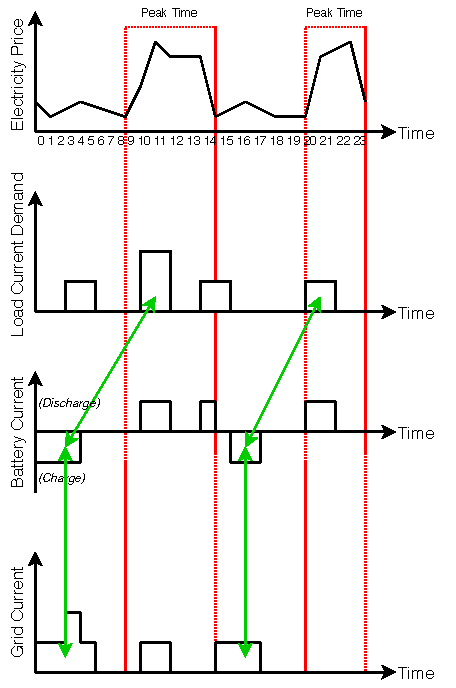
\includegraphics[scale=0.65]{fig/ess.pdf}
%\end{frame}

\section{Weekly progress}
\begin{frame}\frametitle{Autonomous Vehicle (AV) working example}
	\begin{block}{AV system}
		\begin{myitemize}
			\item Small amount of progress made, busy two weeks.
			\item Training system with an increased number of epochs.
			\begin{myitemize}\item Step from 10,000 to 100,000.\end{myitemize}
			\item Altered paper slightly as discussed.
		\end{myitemize}
	\end{block}
\end{frame}

\section{Results}
%\begin{frame}\frametitle{WCRT}
%	\begin{itemize}
%		\item WCRT tests were carried out on various, synchronous systems with SANNs.
%		\item ABRO example utilizing SANNs shown below.
%	\end{itemize}
%	\begin{table}[H]
%		\centering
%		\caption{WCRT results for AI version of ABRO}
%		\label{tbl:res-aibro}
%		\begin{tabular}{|l|l|l|}
%			\hline
%			Approach         & WCRT (ms) & WCET (ms)\\ \hline
%			Black-box        & 2.8  & 2.8  \\ 
%			Layer by layer   & 1.9  & 7.6 \\ 
%			Neuron by neuron & 1.8  & 7.2 \\ \hline
%		\end{tabular}
%	\end{table}
%\end{frame}

%\begin{frame}\frametitle{Meta neural networks}
%	\begin{itemize}
%		\item Using an meta neural network ensemble~\cite{ensembleANN} of SANNs, it was shown that the combined accuracy of 3 SANNs was greater than the accuracy of any one SANN.
%		\item Increase of up to 10\% from individual SANN accuracy.
%		\item Retain synchronous semantics.
%		\item Potential for WCRT analysis. 
%	\end{itemize}
%\end{frame}

\begin{frame} \frametitle{Safe Neural Networks (SNNs) - AV system}
	\begin{table}[t]
		\centering
		\caption{Design and overhead of the policies used in the AV system}
		\label{table:policies}
		\begin{tabular}{|p{0.25\linewidth}|p{0.06\linewidth}|p{0.12\linewidth}|p{0.06\linewidth}|p{0.11\linewidth}|p{0.1\linewidth}|}
			\hline Policy & States & Transitions & Timed & Execution Time (us) & Overhead (\%) \\ \hline   
			%\multicolumn{6}{|p{0.70\linewidth}|}{\ac{AV}} \\ \hline
			$None$ 						& N/A & N/A & N/A & 736 & 0 \\ \hline
			$\varphi_{cnn}$ 			& 1 & 15 & No & 764 & 3.8 \\ \hline
			$\varphi_{drive}$ 			& 1 & 4 & No & 740 & 0.54 \\ \hline
			$\varphi_{car}$ 			& 1 & 7 & No & 741 & 0.66 \\ \hline
			$\varphi_{ped}$ 			& 2 & 56 & Yes & 767 & 4.2 \\ \hline
			$\varphi_{cnn} \wedge \varphi_{drive} \wedge \varphi_{car} \wedge \varphi_{ped}$ 	
			& 2 & 99 & Yes & 803 & 9.1 \\ \hline      
		\end{tabular}
	\end{table}
\end{frame}

\begin{frame} \frametitle{AV System - Not Enforced Results}
	\begin{tabular}{|p{0.15\linewidth}|p{0.15\linewidth}|p{0.15\linewidth}|p{0.15\linewidth}|p{0.15\linewidth}|}
		\hline Number of epochs trained & Percentage accidents & Average minutes to first accident & Average speed (km/h) & Percentage bad brakes \\ \hline
		0 & 100	 & 3.21 & 98 & 19 \\ \hline
		1 & 100 & 3.3 & 93 & 19 \\ \hline
		10 & 100 & 3.8 & 81 & 57 \\ \hline
		100 & 100 & 5.35 & 59 & 24 \\ \hline
		1000 & 100 & 5.31 & 58 & 27 \\  \hline
		10000 & 48.5 & 73.9 & 18 & 63 \\ \hline
		100000 & 91.5 & 39 & 31.5 & 65 \\ \hline                   
	\end{tabular}

	\begin{itemize}
		\item Less than 50\% accidents for the 10,000 epochs trained system
		\begin{itemize}
			\item 220 caused by collision from behind.
			\item 265 otherwise.
		\end{itemize}
	\end{itemize}
\end{frame}
\begin{frame} \frametitle{AV System - Enforced Results}
	\begin{tabular}{|p{0.15\linewidth}|p{0.15\linewidth}|p{0.15\linewidth}|p{0.15\linewidth}|p{0.15\linewidth}|}
		\hline Number of epochs trained & Percentage accidents & Average minutes to first accident & Average speed (km/h) & Percentage bad brakes \\ \hline
		0 & 75.7 & 75.6 & 45 & 0.7 \\ \hline 
		1 & 70.2 & 82.8 & 47 & 4.2 \\ \hline 
		10 & 88.5 & 58.9 & 37 & 20 \\ \hline 
		100 & 79.5 & 72.6 & 41 & 17 \\ \hline 
		1000 & 80.5 & 71.0 & 40 & 18 \\ \hline 
		10000 & 64 & 97.07 & 27.5 & 27 \\ \hline   
		100000 & 57 & 97.14 & 29 & 28 \\ \hline                   
	\end{tabular}

	\begin{itemize}
		\item No accidents caused by fault of the vehicle.
		\begin{itemize}
			\item All caused by a collision from behind.
		\end{itemize}
		\item System managed to finish over 90\% of a run, on average, before the vehicle was hit from behind -- near perfect results.
	\end{itemize}
\end{frame}

\begin{frame} \frametitle{AV System - Results}
	\begin{figure}[t]
		\centering
		\scalebox{1}{\begin{tikzpicture}
	\begin{loglogaxis}[
	xlabel={Number of epochs trained},
	ylabel={Time to first incident (/100)},
	x=0.8cm,
	y=1.2cm, 
	legend style={at={(0.1,0.55)},anchor=west}]
	
	\addplot[color=blue,mark=*] coordinates {
		(0,3.24)
		(1,3.29)
		(10,3.78)
		(100,5.53)
		(1000,5.74)
		(10000,27.41)
	};

	\addplot[color=red,mark=x] coordinates {
		(0,93.2)
		(1,94.5)
		(10,91.91)
		(100,94.5)
		(1000,94.2)
		(10000,96.69)
	};

	\legend{Policies not enforced, Policies enforced}
	\end{loglogaxis}%
\end{tikzpicture}%}
		\caption{Line graph showing the performance of the enforced system compared to the un-enforced system \label{fig:avgraph}}
	\end{figure}
\end{frame}

\begin{frame} \frametitle{AV System - Results}
	\begin{myitemize}
		\item Re-structured GA to produce better results.
		\item The training sweet spot is around 10,000 epochs.
		\item Over-training the system results in reduced performance.
		\begin{myitemize}
			\item Over-fitting training data.
			\item GA fitness function not perfect.
		\end{myitemize}
		\item Over-training has no prominent affect on the enforced results.
	\end{myitemize}
\end{frame}

\begin{frame} \frametitle{Keras Parser}
	\begin{myitemize}
		\item Installed and learned the basics of Keras w/ Tensorflow back-end.
		\begin{myitemize}
			\item Created and trained basic XOR MLP.
		\end{myitemize}
		\item Created a parser that takes in a JSON model file and a HDF5 weight file.
		\begin{myitemize}
			\item Parses the model structure and weights and maps them to a Python class.
			\item Functionality to view the structure and weights.
			\item Can generate a C array of weights that can be used to init a C ANN.
		\end{myitemize}
		\item Successfully parsed and mapped a trained MLP (XOR) to C.
		\begin{myitemize}
			\item Correlation coefficient: 99.99942\%
		\end{myitemize}
	\end{myitemize}
\end{frame}

\begin{frame} \frametitle{Keras Parser}
	\begin{block}{What is important to parse?}
		\begin{myitemize}
			\item Number of layers.
			\item Type of layer (dense, convolutional, dropout, etc).
			\item Activation functions (ReLu, sigmoid, etc).
			\item Number and type of inputs and outputs.
			\item Number of weights per layer.
			\item Weight values.
		\end{myitemize}
	\end{block}
\end{frame}

%\begin{frame} \frametitle{New case study -- IoT intrusion detection}
%	\begin{block}{IoT is cyber-physical and (possibly) safety-critical}
%		\begin{myitemize}
%			\item IoT is a network of physical devices (i.e. CPS).
%			\item Extends the Internet beyond standard devices.
%			\item Vulnerable to intrusion -- safety implications.
%			\item Various types of intrusion detection algorithms.
%			\begin{myitemize}
%				\item Host-based.
%				\item Network-based.
%			\end{myitemize}
%			\item Propose SNNs for intrusion detection on IoT devices.
%		\end{myitemize}
%	\end{block}
%\end{frame}

%\begin{frame} \frametitle{New case study -- Drone control}
%	\begin{block}{Avalanche victim rescue drone~\cite{dickensheets2015}}
%		\begin{myitemize}
%			\item Autonomous drone to locate avalanche victims by following a radio signal.
%			\item Safety critical system.
%			\begin{myitemize}
%				\item Failure to find the victim can lead to their death.
%				\item Crashing of the drone can be dangerous to unaware people.
%			\end{myitemize}
%			\item Drone navigation can be improved and made safe using SNNs.
%			\begin{myitemize}
%				\item Advanced controller network.
%				\item Prevent unsafe behaviour.
%			\end{myitemize}
%		\end{myitemize}
%	\end{block}
%\end{frame}

%\begin{frame} \frametitle{New case study -- Drone control}
%	\begin{block}{Avalanche victim rescue drone~\cite{dickensheets2015}}
%		\begin{myitemize}
%			\item Location of radio signal origin unknown.
%			\item ANN to find radio signal and navigate obstacles.
%			\item RE for obstacle avoidance and navigation.
%			\begin{myitemize}
%				\item Drone must not crash.
%				\item Drone must go in the correct direction.
%			\end{myitemize}
%			\item ANNs to recognise objects.
%		\end{myitemize}
%	\end{block}
%\end{frame}

%\begin{frame} \frametitle{New case study -- Drone control}
%	\begin{figure}[t]
%		\centering
%		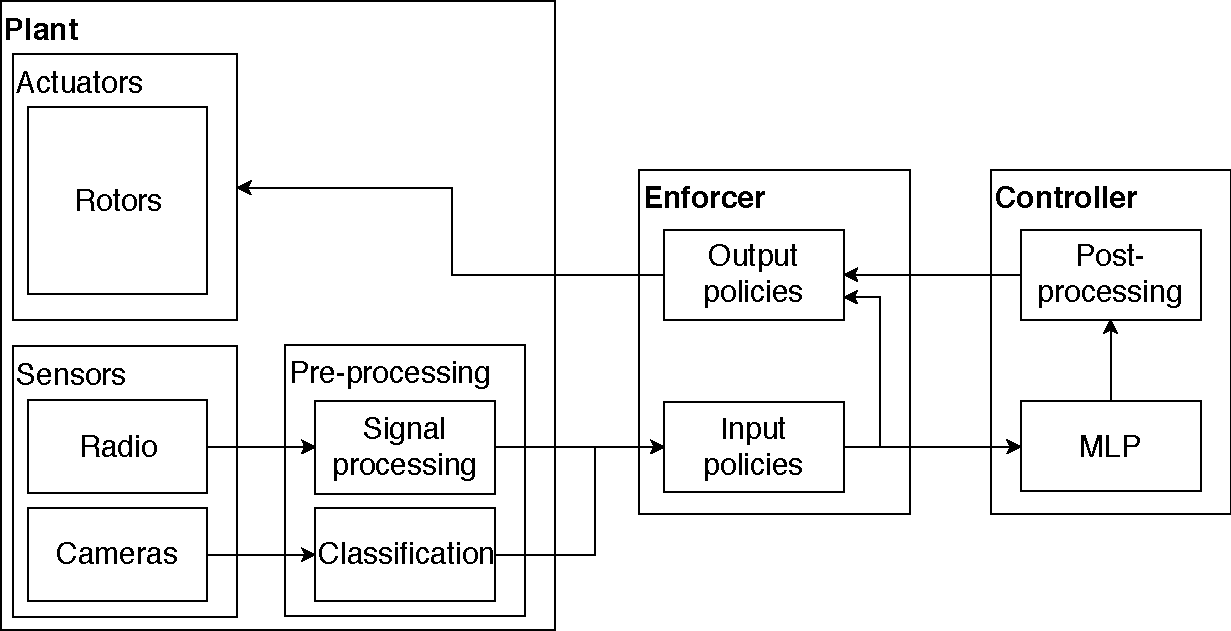
\includegraphics[width=\linewidth]{fig/drone-sys.pdf}
%		\caption{Block diagram for the drone safety system. \label{fig:dronesys}}
%	\end{figure}
%\end{frame}

%\begin{frame} \frametitle{New case study -- Drone control}
%	\begin{figure}[t]
%		\centering
%		\scalebox{0.7}{

\begin{tikzpicture}[>=stealth',shorten >=1pt,auto,node distance=4 cm, scale = 1, transform shape]

\tikzstyle{accept} = [draw=blue!75,fill=blue!20]
\tikzstyle{violate} = [draw=red!75,fill=red!20]

\node[initial,state, accepting, accept] (A) {$q_{hot}$};
\node[state, accepting, accept] (B) [right of=A] {$q_{cold}$};
\node[state, accepting, accept] (D) [right of=B] {$q_{found}$};
\node[state, violate]         (C) [below of=B]  {$q_v$};

\path[->] 
		(A) edge [loop above]       node [above, xshift=-1em]  
		{
			\scriptsize$\let\scriptstyle\textstyle\substack{(S~>~\mathbf{S})~\&~\\~}$
		} (A)
		
		(A) edge [bend left=45]		node [above]  
		{
			\scriptsize$\let\scriptstyle\textstyle\substack{}$
		} (B)
	
		(A) edge [bend right=70]	node [above]  
		{
			\scriptsize$\let\scriptstyle\textstyle\substack{}$
		} (C)
	
		(B) edge [loop above]		node [above, xshift=2em]  
		{
			\scriptsize$\let\scriptstyle\textstyle\substack{}$
		} (B)
	
		(B) edge [left]				node [below]  
		{
			\scriptsize$\let\scriptstyle\textstyle\substack{}$
		} (A)
		
		(B) edge [right]			node [below]  
		{
			\scriptsize$\let\scriptstyle\textstyle\substack{}$
		} (C)
	
		(C) edge [loop below]		node [below]  
		{
			\scriptsize$\sum$
		} (C)
		;

\end{tikzpicture}}
%		\caption{Enforcer policy for the autonomous drone control \label{fig:dronerte}}
%	\end{figure}
%\end{frame}



\begin{frame}\frametitle{Final thesis chapter -- Introduction \& Background}
	\begin{myitemize}
		\item Deep ANNs with large, complex inputs are very hard to verify~\cite{Gehr2018AI2SA}.
		\item These ANNs, namely CNNs, are susceptible to input perturbations~\cite{Gehr2018AI2SA, ann-pert}, further increasing the difficulty of verification.
		\item Previously introduced RE (Runtime Enforcement) techniques cannot handle these complex inputs.
		\item Propose sensor fusion and a MNN ensemble.
		\begin{myitemize}
			\item Sensor fusion~\cite{SensorFusion2017} allows RE based on the inputs to the system.
			\item MNN increases prediction accuracy by using multiple, different CNNs for the same job.
		\end{myitemize}
	\end{myitemize}
\end{frame}


\begin{frame}\frametitle{Final thesis chapter -- Case Study}
	\begin{myitemize}
		\item Autonomous Vehicle research growing rapidly.
		\item Systems not perfect, accidents do happen and can be fatal~\cite{coldewey_2018}.
		\item Proposed solution for accidents such as~\cite{coldewey_2018}.
		\begin{myitemize}
			\item Increase prediction accuracy.
			\item Runtime verification of the system.
		\end{myitemize}
	\item Simulation of the system is needed.
	\end{myitemize}
\end{frame}

\begin{frame}\frametitle{Final thesis chapter -- Methodology}
	\begin{myitemize}
		\item System consists of:
		\begin{myitemize}
			\item Complex, Meta Neural Network ensemble to classify the input images.
			\item LiDAR to support the MNN.
			\item Safety policy to prevent unsafe classifications.
			\item Runtime Enforcer to enforce safety policy.
		\end{myitemize}
	\end{myitemize}
\end{frame}

\begin{frame}\frametitle{Final thesis chapter -- Methodology}
	\begin{myitemize}
		\item System consists of:
		\begin{myitemize}
			\item Complex, Meta Neural Network ensemble to classify the input images.
			\item LiDAR to support the MNN.
			\item Safety policy to prevent unsafe classifications.
			\item Runtime Enforcer to enforce safety policy.
		\end{myitemize}
	\end{myitemize}
\end{frame}

\begin{frame} \frametitle{Final thesis chapter -- MNN}
	\begin{block}{The Meta Neural Network in question}
		\begin{figure}[t]
			\centering
			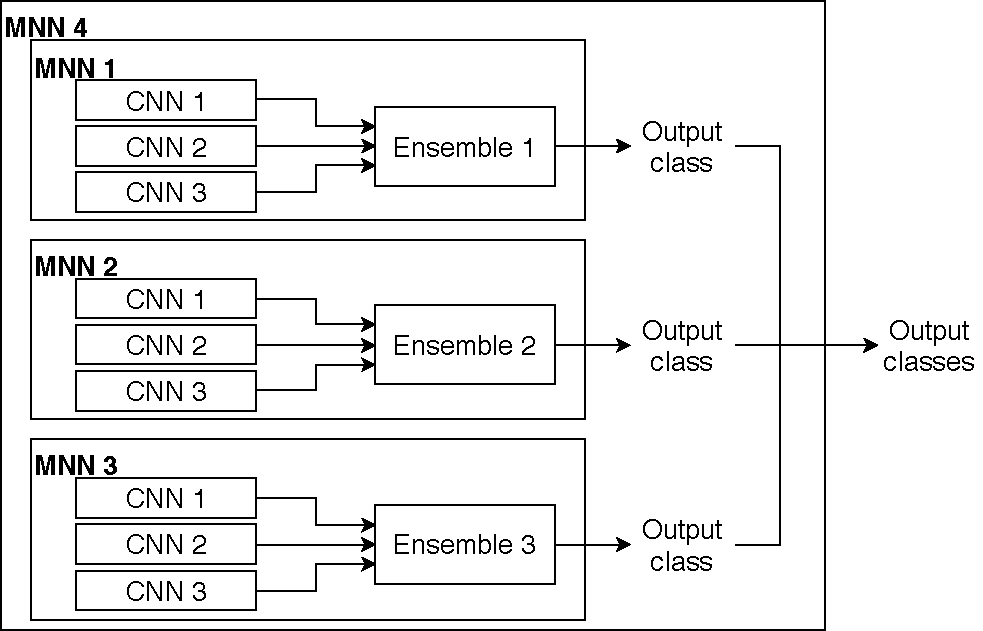
\includegraphics[scale=0.5]{fig/MNN.pdf}
			\caption{Block diagram showing the Meta Neural Network ensemble. \label{fig:mnn}}
		\end{figure}
	\end{block}
\end{frame}

\begin{frame} \frametitle{Final thesis chapter -- Safety policy}
	\begin{block}{The enforced policy in question}
		\begin{myitemize}
			\item $P$ -- Misclassification of a person relative to the LiDAR output.
			\item $C$ -- Misclassification of a car relative to the LiDAR output.
			\item $N$ -- Misclassification of nothing relative to the LiDAR output.
			\item $S$ -- Misclassification of a sign relative to the LiDAR output.
			\item $C$ -- Confidence of the object.
			\item $t$ -- Tick counter for manual control.
		\end{myitemize}
	\end{block}	
\end{frame}

\begin{frame} \frametitle{Final thesis chapter -- Safety policy (cont.)}
	\begin{block}{The enforced policy in question}
		\begin{figure}[t]
			\centering
			\scalebox{0.8}{

\begin{tikzpicture}[>=stealth',shorten >=1pt,auto,node distance=6 cm, scale = 1, transform shape]

\tikzstyle{accept} = [draw=blue!75,fill=blue!20]
\tikzstyle{violate} = [draw=red!75,fill=red!20]

\node[initial,state, accepting, accept] (A) {$q_{safe}$};
\node[state, violate]         (B) [right of=A]  {$q_v$};

\path[->] 
		(A) edge [loop above]       node [above, xshift=-1em]  
		{
			\scriptsize$\let\scriptstyle\textstyle\substack{
			\sum~\textbackslash~\\
			\Big((L~=~0)~\&~(\overline{O~=~0})~\&~(S~<~90)~|~\\~
			(L~=~1)~\&~(\overline{O~=~1})~\&~(S~<~90)~|~\\
			(L~=~2)~\&~(\overline{O~=~2})~\&~(S~<~90)\Big)}$
		} (A)
		
		(A) edge [left]		node [below]  
		{
			\scriptsize$\let\scriptstyle\textstyle\substack{
			(L~=~0)~\&~(\overline{O~=~0})~\&~(S~<~90)~|~\\~
			(L~=~1)~\&~(\overline{O~=~1})~\&~(S~<~90)~|~\\
			(L~=~2)~\&~(\overline{O~=~2})~\&~(S~<~90)}$
		} (B)
	
		(B) edge [loop above]		node [above]  
		{
			\scriptsize$\sum$
		} (B)
		;

\end{tikzpicture}}
			\caption{Enforcer policy for the AV prediction \label{fig:signrte}}
		\end{figure}
	\end{block}
\end{frame}

\begin{frame} \frametitle{Final thesis chapter -- Overall system}
	\begin{block}{The Safe Synchronous Neural Network as a whole}
		\begin{figure}[t]
			\centering
			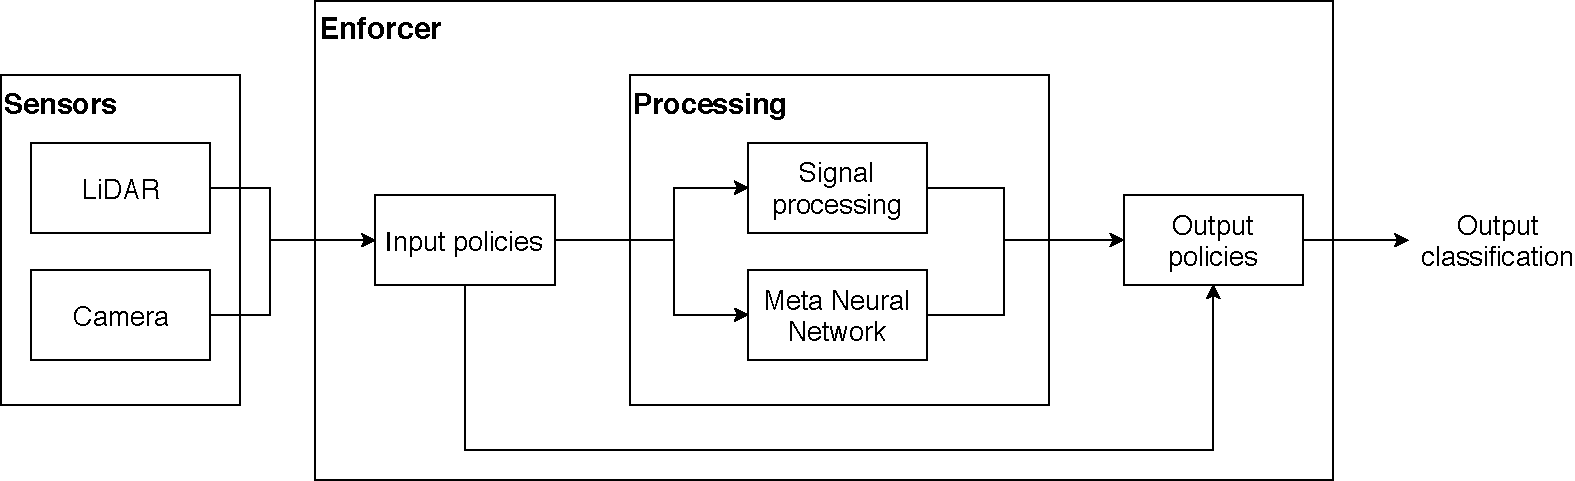
\includegraphics[width=\linewidth]{fig/SSNN.pdf}
			\caption{Figure showing the SSNN used in the AV prediction system \label{fig:snn}}
		\end{figure}
	\end{block}
\end{frame}

\begin{frame} \frametitle{Final thesis chapter -- Results}
	\begin{table}[h]
		\centering
		\resizebox{\textwidth}{!}{%
		\begin{tabular}{|p{0.17\linewidth}||p{0.17\linewidth}|p{0.17\linewidth}|p{0.17\linewidth}|p{0.17\linewidth}|}
			\hline
			Object classified & No. of misclassifications (\%) & Caught misclassifications (\%) & False negatives (\%) & Total remaining misclassifications (\%) \\ \hline
			Person & 17.01 & 17.01 & 0.00 & 0.00 \\ \hline
			Vehicle & 15.85 & 15.85 & 0.00 & 0.00 \\ \hline
			Sign & 54.46 & 54.46 & 4.84 & 4.84 \\ \hline
			Nothing & 7.83 & 7.83 & 0.00 & 0.00 \\ \hline
			All & 95.16 & 95.16 & 4.84 & 4.84 \\ \hline
		\end{tabular}%
		}
		\caption{Table showing the worst results of the AV prediction SNN using the original images, trained for 0 epochs}
		\label{tbl:sign-res1}
	\end{table}
\end{frame}

\begin{frame} \frametitle{Final thesis chapter -- Results}
	\begin{table}[h]
		\centering
		\resizebox{\textwidth}{!}{%
		\begin{tabular}{|p{0.17\linewidth}||p{0.17\linewidth}|p{0.17\linewidth}|p{0.17\linewidth}|p{0.17\linewidth}|}
			\hline
			Object classified & No. of misclassifications (\%) & Caught misclassifications (\%) & False negatives (\%) & Total remaining misclassifications (\%) \\ \hline
			Person & 1.00 & 0.21 & 0.53 & 1.32 \\ \hline
			Vehicle & 6.26 & 5.63 & 0.44 & 1.07 \\ \hline
			Sign & 2.62 & 0.44 & 1.02 & 3.20 \\ \hline
			Nothing & 2.50 & 2.27 & 0.12 & 0.35 \\ \hline
			All & 12.38 & 8.55 & 2.11 & 5.93 \\ \hline
		\end{tabular}%
		}
		\caption{Table showing results of the AV prediction SNN using the original images, trained for 10000 epochs}
		\label{tbl:sign-res10000}
	\end{table}
\end{frame}

\begin{frame} \frametitle{Final thesis chapter -- Results}
	\begin{table}[h]
		\centering
		\resizebox{\textwidth}{!}{%
		\begin{tabular}{|p{0.17\linewidth}||p{0.17\linewidth}|p{0.17\linewidth}|p{0.17\linewidth}|p{0.17\linewidth}|}
			\hline
			Object classified & No. of misclassifications (\%) & Caught misclassifications (\%) & False negatives (\%) & Total remaining misclassifications (\%) \\ \hline
			Person & 17.01 & 17.01 & 0.00 & 0.00 \\ \hline
			Vehicle & 15.85 & 15.85 & 0.00 & 0.00 \\ \hline
			Sign & 54.46 & 54.46 & 4.84 & 4.84 \\ \hline
			Nothing & 7.83 & 7.83 & 0.00 & 0.00 \\ \hline
			All & 95.16 & 95.16 & 4.84 & 4.84 \\ \hline
		\end{tabular}%
		}
		\caption{Table showing the worst results of the AV prediction SNN using perturbed images, trained for 0 epochs}
		\label{tbl:sign-respert1}
	\end{table}
\end{frame}

\begin{frame} \frametitle{Final thesis chapter -- Results}
	\begin{table}[h]
		\centering
		\resizebox{\textwidth}{!}{%
		\begin{tabular}{|p{0.17\linewidth}||p{0.17\linewidth}|p{0.17\linewidth}|p{0.17\linewidth}|p{0.17\linewidth}|}
			\hline
			Object classified & No. of misclassifications (\%) & Caught misclassifications (\%) & False negatives (\%) & Total remaining misclassifications (\%) \\ \hline
			Person & 3.43 & 0.60 & 0.56 & 3.38 \\ \hline
			Vehicle & 10.78 & 8.57 & 0.23 & 2.43 \\ \hline
			Sign & 38.08 & 31.91 & 1.39 & 7.56 \\ \hline
			Nothing & 5.61 & 4.80 & 0.09 & 0.90 \\ \hline
			All & 57.89 & 45.89 & 2.27 & 14.28 \\ \hline
			\end{tabular}%
		}
		\caption{Table showing results of the AV prediction SNN using perturbed images, trained for 10000 epochs}
		\label{tbl:sign-respert10000}
	\end{table}
\end{frame}


\begin{frame} \frametitle{Final thesis chapter -- Results}
	\begin{figure}[t]
		\centering
		\scalebox{0.5}{\begin{tikzpicture}
\begin{semilogxaxis}[
xlabel={Number of epochs trained},
ylabel={System classification accuracy (\%)},
x=1.3cm,
y=1.0mm, 
legend style={at={(0.02,0.55)},anchor=west}]

\addplot[color=brown,mark=x] coordinates {
	(1, 100 - 95.159996)
	(10, 100 - 95.159996)
	(20, 100 - 95.300003)
	(30, 100 - 94.410004)
	(40, 100 - 94.180000)
	(50, 100 - 95.019997)
	(60, 100 - 94.389999)
	(70, 100 - 93.000000)
	(80, 100 - 93.419998)
	(90, 100 - 94.159996)
	(100, 100 - 82.669998)
	(200, 100 - 59.790001)
	(300, 100 - 39.240002)
	(400, 100 - 25.930000)
	(500, 100 - 27.490000)
	(600, 100 - 22.389999)
	(700, 100 - 14.180000)
	(800, 100 - 15.390000)
	(900, 100 - 12.700000)
	(1000, 100 - 29.359999)
	(2000, 100 - 15.460000)
	(3000, 100 - 14.810000)
	(4000, 100 - 14.390000)
	(5000, 100 - 13.490000)
	(6000, 100 - 10.590000)
	(7000, 100 - 12.400000)
	(8000, 100 - 18.889999)
	(9000, 100 - 10.920000)
	(10000, 100 - 12.380000)
};

\addplot[color=black,mark=x] coordinates {
	(1, 100 - 4.840000)
	(10, 100 - 4.840000)
	(20, 100 - 4.630000)
	(30, 100 - 5.470000)
	(40, 100 - 5.700000)
	(50, 100 - 4.910000)
	(60, 100 - 5.610000)
	(70, 100 - 6.980000)
	(80, 100 - 5.910000)
	(90, 100 - 5.520000)
	(100, 100 - 23.410000)
	(200, 100 - 22.780001)
	(300, 100 - 14.000000)
	(400, 100 - 12.310000)
	(500, 100 - 10.570000)
	(600, 100 - 10.960000)
	(700, 100 - 7.790000)
	(800, 100 - 8.410000)
	(900, 100 - 7.020000)
	(1000, 100 - 10.890000)
	(2000, 100 - 7.530000)
	(3000, 100 - 7.000000)
	(4000, 100 - 7.090000)
	(5000, 100 - 6.490000)
	(6000, 100 - 5.310000)
	(7000, 100 - 5.680000)
	(8000, 100 - 8.640000)
	(9000, 100 - 6.810000)
	(10000, 100 - 5.930000)
};

\legend{Policies not enforced, Policies enforced}
\end{semilogxaxis}%
\end{tikzpicture}%}
		\caption{Line graph showing the performance of the system trained over an increasing amount of epochs using unperturbed inputs \label{fig:sign-graph}}
	\end{figure}
\end{frame}

\begin{frame} \frametitle{Final thesis chapter -- Results}
	\begin{figure}[t]
		\centering
		\scalebox{0.5}{\begin{tikzpicture}
\begin{semilogxaxis}[
xlabel={Number of epochs trained},
ylabel={Overall miscalssifications made by the system (\%)},
x=1.3cm,
y=1.0mm, 
legend style={at={(0.02,0.55)},anchor=west}]

\addplot[color=blue,mark=*] coordinates {
	(1, 100 - 95.156433)
	(10, 100 - 95.156433)
	(20, 100 - 97.450752)
	(30, 100 - 96.454231)
	(40, 100 - 94.831978)
	(50, 100 - 95.527229)
	(60, 100 - 95.179604)
	(70, 100 - 94.090385)
	(80, 100 - 95.086906)
	(90, 100 - 95.156433)
	(100, 100 - 93.626884)
	(200, 100 - 83.754349)
	(300, 100 - 76.732330)
	(400, 100 - 72.236382)
	(500, 100 - 70.892235)
	(600, 100 - 72.862106)
	(700, 100 - 52.537659)
	(800, 100 - 61.251450)
	(900, 100 - 54.275784)
	(1000, 100 - 76.685982)
	(2000, 100 - 59.953651)
	(3000, 100 - 57.798378)
	(4000, 100 - 61.112400)
	(5000, 100 - 61.251450)
	(6000, 100 - 56.523754)
	(7000, 100 - 60.417149)
	(8000, 100 - 67.902664)
	(9000, 100 - 57.497105)
	(10000, 100 - 57.891079)
};

\addplot[color=red,mark=*] coordinates {
	(1, 100 - 4.843569)
	(10, 100 - 4.843569)
	(20, 100 - 2.549247)
	(30, 100 - 3.545771)
	(40, 100 - 5.144844)
	(50, 100 - 4.495944)
	(60, 100 - 4.820394)
	(70, 100 - 5.909617)
	(80, 100 - 4.727694)
	(90, 100 - 4.843569)
	(100, 100 - 22.294323)
	(200, 100 - 18.331402)
	(300, 100 - 13.603708)
	(400, 100 - 15.249131)
	(500, 100 - 13.534184)
	(600, 100 - 16.546928)
	(700, 100 - 14.623406)
	(800, 100 - 15.805330)
	(900, 100 - 14.831982)
	(1000, 100 - 14.229432)
	(2000, 100 - 14.669757)
	(3000, 100 - 14.252607)
	(4000, 100 - 14.275783)
	(5000, 100 - 14.646582)
	(6000, 100 - 15.017382)
	(7000, 100 - 13.487833)
	(8000, 100 - 14.507532)
	(9000, 100 - 13.858633)
	(10000, 100 - 14.275783)
};

\legend{Policies not enforced, Policies enforced}
\end{semilogxaxis}%
\end{tikzpicture}%}
		\caption{Line graph showing the number of misclassifications made by the system with perturbed inputs \label{fig:sign-graphpert}}
	\end{figure}
\end{frame}

\begin{frame} \frametitle{Final thesis chapter -- Results}
	\begin{figure}[t]
		\centering
		\scalebox{0.5}{\begin{tikzpicture}
\begin{semilogxaxis}[
xlabel={Number of epochs trained},
ylabel={Overall miscalssifications made by the system (\%)},
x=1.3cm,
y=1.0mm, 
legend style={at={(0.02,0.55)},anchor=west}]

\addplot[color=blue,mark=*] coordinates {
	(1, 100 - 95.156433) 
	(10, 100 - 95.156433)
	(20, 100 - 97.450752)
	(30, 100 - 96.454231)
	(40, 100 - 94.831978)
	(50, 100 - 95.527229)
	(60, 100 - 95.179604)
	(70, 100 - 94.090385)
	(80, 100 - 95.086906)
	(90, 100 - 95.156433)
	(100, 100 - 93.626884)
	(200, 100 - 83.754349)
	(300, 100 - 76.732330)
	(400, 100 - 72.236382)
	(500, 100 - 70.892235)
	(600, 100 - 72.862106)
	(700, 100 - 52.537659)
	(800, 100 - 61.251450)
	(900, 100 - 54.275784)
	(1000, 100 - 76.685982)
	(2000, 100 - 59.953651)
	(3000, 100 - 57.798378)
	(4000, 100 - 61.112400)
	(5000, 100 - 61.251450)
	(6000, 100 - 56.523754)
	(7000, 100 - 60.417149)
	(8000, 100 - 67.902664)
	(9000, 100 - 57.497105)
	(10000, 100 - 57.891079)
};

\addplot[color=red,mark=*] coordinates {
	(1, 100 - 4.843569)
	(10, 100 - 4.843569)
	(20, 100 - 2.549247)
	(30, 100 - 3.545771)
	(40, 100 - 5.144844)
	(50, 100 - 4.495944)
	(60, 100 - 4.820394)
	(70, 100 - 5.909617)
	(80, 100 - 4.727694)
	(90, 100 - 4.843569)
	(100, 100 - 22.294323)
	(200, 100 - 18.331402)
	(300, 100 - 13.603708)
	(400, 100 - 15.249131)
	(500, 100 - 13.534184)
	(600, 100 - 16.546928)
	(700, 100 - 14.623406)
	(800, 100 - 15.805330)
	(900, 100 - 14.831982)
	(1000, 100 - 14.229432)
	(2000, 100 - 14.669757)
	(3000, 100 - 14.252607)
	(4000, 100 - 14.275783)
	(5000, 100 - 14.646582)
	(6000, 100 - 15.017382)
	(7000, 100 - 13.487833)
	(8000, 100 - 14.507532)
	(9000, 100 - 13.858633)
	(10000, 100 - 14.275783)
};

\addplot[color=brown,mark=x] coordinates {
	(1, 100 - 95.159996)
	(10, 100 - 95.159996)
	(20, 100 - 95.300003)
	(30, 100 - 94.410004)
	(40, 100 - 94.180000)
	(50, 100 - 95.019997)
	(60, 100 - 94.389999)
	(70, 100 - 93.000000)
	(80, 100 - 93.419998)
	(90, 100 - 94.159996)
	(100, 100 - 82.669998)
	(200, 100 - 59.790001)
	(300, 100 - 39.240002)
	(400, 100 - 25.930000)
	(500, 100 - 27.490000)
	(600, 100 - 22.389999)
	(700, 100 - 14.180000)
	(800, 100 - 15.390000)
	(900, 100 - 12.700000)
	(1000, 100 - 29.359999)
	(2000, 100 - 15.460000)
	(3000, 100 - 14.810000)
	(4000, 100 - 14.390000)
	(5000, 100 - 13.490000)
	(6000, 100 - 10.590000)
	(7000, 100 - 12.400000)
	(8000, 100 - 18.889999)
	(9000, 100 - 10.920000)
	(10000, 100 - 12.380000)
};

\addplot[color=black,mark=x] coordinates {
	(1, 100 - 4.840000)
	(10, 100 - 4.840000)
	(20, 100 - 4.630000)
	(30, 100 - 5.470000)
	(40, 100 - 5.700000)
	(50, 100 - 4.910000)
	(60, 100 - 5.610000)
	(70, 100 - 6.980000)
	(80, 100 - 5.910000)
	(90, 100 - 5.520000)
	(100, 100 - 23.410000)
	(200, 100 - 22.780001)
	(300, 100 - 14.000000)
	(400, 100 - 12.310000)
	(500, 100 - 10.570000)
	(600, 100 - 10.960000)
	(700, 100 - 7.790000)
	(800, 100 - 8.410000)
	(900, 100 - 7.020000)
	(1000, 100 - 10.890000)
	(2000, 100 - 7.530000)
	(3000, 100 - 7.000000)
	(4000, 100 - 7.090000)
	(5000, 100 - 6.490000)
	(6000, 100 - 5.310000)
	(7000, 100 - 5.680000)
	(8000, 100 - 8.640000)
	(9000, 100 - 6.810000)
	(10000, 100 - 5.930000)
};

\legend{Policies not enforced (perturbed), Policies enforced (perturbed), Policies not enforced (perturbations), Policies enforced (perturbations)}
\end{semilogxaxis}%
\end{tikzpicture}%}
		\caption{Line graph showing the number of misclassifications made by the system over all inputs \label{fig:sign-graphboth}}
	\end{figure}	
\end{frame}

\begin{frame} \frametitle{Final thesis chapter -- Discussion}
	\begin{myitemize}
		\item First, input perturbations greatly decrease the prediction accuracy of the system.
		\item Second, the enforcer increases the accuracy of the system, both with and without input perturbations.
		\item Third, the enforcer's performance remains fairly steady across the entire range of trained epochs.
		\begin{myitemize}
			\item The best results were found when the CNNs were not trained much.
			\item This is due to the system taking the accuracy of the LiDAR when the CNNs in use are not confident about their outputs.
			\item As the CNNs are trained more, the performance decreases from its original peak. 
			\item This is because the error of the CNNs are taken in to consideration in addition to the error of the LiDAR, since trained CNNs are more confident of their predictions.
		\end{myitemize} 
	\end{myitemize}
\end{frame}

\begin{frame} \frametitle{Final thesis chapter -- Conclusion}
	\begin{myitemize}
		\item The enforcer does increase the overall classification accuracy of the system. 
		\item When the system is untrained, the system is as accurate as the LiDAR.
		\item In a system with more variation in object types, this will be much less accurate, since the LiDAR will be less reliable.
		\item When the system is fully trained, the overall classification accuracy is still increased far beyond the accuracy without the enforcer.
		\item With CNNs that are better trained, with more time and resources, the overall accuracy of the system should increase beyond that of an untrained system.
	\end{myitemize}
\end{frame}

\begin{frame}\frametitle{Final thesis chapter -- TODO}
	\begin{block}{Create other version of the system}
		\begin{myitemize}
			\item ANN to do sensor fusion in place of the enforcer.
			\item Show how system performs with an ANN in place of the enforcer.
		\end{myitemize}
	\end{block}
	\begin{block}{Add Keras2C ANNs to system and train using Python}
		\begin{myitemize}
			\item Use Marc's compiler to train and add CNNs to the system in place of the current Darknet CNNs.
			\item Performance difference?
		\end{myitemize}
	\end{block}
	\begin{block}{Finish writing chapter}
		\begin{myitemize}
			\item Ditto.
		\end{myitemize}
	\end{block}
\end{frame}











\begin{frame} \frametitle{Table -- possible ANN systems}
	\vspace{2cm}
	\begin{table}[]
		\centering
		\resizebox{\textwidth}{!}{%
			\begin{tabular}{|l|l|l|l|l|l|l|}
				\hline
				Name                     & Source & Deadline strictness & Consequence of missed deadline & Examples of failure & Real world interactivity & Network types \\ \hline
				Autonomous vehicle  & & & & & & \\ \hline
				Disease detection & & & & & & \\ \hline 
				Smart grid & & & & & & \\ \hline 
				Behaviour modeling & & & & & & \\ \hline 
				Malware detection & & & & & & \\ \hline 
				Forex & & & & & & \\ \hline
				Smart factory & & & & & & \\ \hline
				Internet of Things & & & & & & \\ \hline
				Drone control & & & & & & \\ \hline
			\end{tabular}%
		}
		\caption{My caption}
		\label{my-label}
	\end{table}
\end{frame}

\section{Conclusion}
\begin{frame}\frametitle{Future work -- Final Master's sections}
	\begin{block}{Import Keras ANNs into C + Esterel SNNs}
		\begin{myitemize}
			\item 
		\end{myitemize}
	\end{block}
	\begin{block}{Realistic AV model}
		\begin{myitemize}
			\item 
		\end{myitemize}
	\end{block}
\end{frame}

%\begin{frame}[allowframebreaks]	
%	\printbibliography
%\end{frame}

\begin{frame}[allowframebreaks] \frametitle{References}
	\bibliographystyle{ieeetr}
	\bibliography{references} 
\end{frame}

\appendix

\end{document}